\documentclass{memoir}
\usepackage{stmaryrd}
\usepackage{lscape}
\usepackage{hyperref}
\usepackage{nameref}
\usepackage[pdftex]{graphicx}
\usepackage{hyperref}
\hypersetup{
    bookmarks=true,         % show bookmarks bar?
    unicode=false,          % non-Latin characters in Acrobat�s bookmarks
    pdftoolbar=true,        % show Acrobat�s toolbar?
    pdfmenubar=true,        % show Acrobat�s menu?
    pdffitwindow=true,      % page fit to window when opened
%   pdftitle={My title},    % title
%   pdfauthor={Author},     % author
%   pdfsubject={Subject},   % subject of the document
    pdfnewwindow=true,      % links in new window
%   pdfkeywords={keywords}, % list of keywords
    colorlinks=true,        % false: boxed links; true: colored links
    linkcolor=blue,         % color of internal links
    citecolor=blue,         % color of links to bibliography
    filecolor=blue,         % color of file links
    urlcolor=blue           % color of external links
}

\usepackage{xcolor}
\usepackage{listings}
\lstset{language=C++}

\lstset{basicstyle=\ttfamily,
  showstringspaces=false,
  commentstyle=\color{red},
  keywordstyle=\color{blue}
}

\oddsidemargin80pt      %commentare se si stampa solo fronte
\evensidemargin40pt     %commentare se si stampa solo fronte


\begin{document}

\frontmatter

%\thispagestyle{empty}

\newcommand{\HS}[1][1.]{\hspace{\stretch{#1}}}
\begin{center}

%\begin{figure}
%\centerline{\psfig{figure=logouni.eps}}
%\end{figure}

\huge{UNIVERSITY OF CALABRIA}\\
\vspace*{0.25cm}
\large{Department of Mathematics}\\
\normalsize{Via P. Bucci\\
I-87036 Rende, Italy\\
\vspace*{0.25cm} \HS \hrulefill \HS}

%\large{Internal Report 02/2009}\\


\vspace*{3.5cm}

\Large{\textbf{User Guide to the OpenCAL - The open Cellular Automata
Library - }\\
\vspace*{0.5cm}
\Large{\textbf{Version 1.0}}
\vspace*{1cm}

%\normalsize{by}

\vspace*{1cm}

%\normalsize{\textit{Giuseppe Spingola, Giuseppe Zito, Donato D'Ambrosio,
% William Spataro and Rocco Rongo}}

\vspace*{3.5cm}

\normalsize{September, 2009}

\vspace*{2.0cm}

%\footnotesize{This work was supported by the Department of Mathematics of
% University of Calabria. Parallel computer machineries were provided by the High Performance Computing Center of the same University.}

%\HS[.1] \hrulefill \hspace*{1.5cm} \\
%\quad \normalsize A.A. 2002-2003 \quad

\end{center}

%\chapter*{Acknowledgements}


\emph{We are gratefull to all OpenCAL developers and supporters.\\
  In particular, we acknowledge Francesca ``Chesire Cat''
  Aceto, Luigi Olivella, Paola ``AruQ'' Arcuri, Carmelo La Gamba, Maurizio
  Macri', Marco ``Pecos'' Oliverio, Rocco ``Rick'' Rongo, Alfonso Senatore, and
  Mario ``Suinos'' D'Onghia.}

\newpage



\newpage

\pagenumbering{roman}

\tableofcontents

\pagenumbering{arabic}

%\chapter{Introduction}

OpenCAL (Open Computing Abstraction Layer) is a parallel computational
software library, developed as an Open Source project at the
Department of Mathematics and Computer Science University of Calabria
(Italy) and released under the LGPL v2.1 license.

OpenCAL allows for the definition of numerical simulation models based
on the Cellular Automata computational paradigm. It also supports
eXtended Cellular Automata (XCA), the Finite Differences method and,
in general, all numerical methods based on uniform computational
grids.

OpenCAL is currently developed in C/C++ and can run in parallel on
both CPUs, thanks to its implementation based on OpenMP, and on GPUs,
thanks to its implementation in OpenCL.

%% Cellular Automata (CA) represent a parallel computing methodology for
%% modelling complex systems. Well known examples of applications include
%% the simulation of natural phenomena such as lava and debris flows,
%% forest fires, agent based social processes such as pedestrian
%% evacuation and highway traffic problems, besides many others (e.g.,
%% theoretical studies).

%% Many Cellular Automata software environments and libraries exist.
%% However, when non-trivial modelling is needed, only non-open source
%% software are generally available. This is particularly true for
%% eXtended Cellular Automata (XCA), adopted for simulating phenomena at
%% a macroscopic point of view, for which only a significant example of
%% non free software exists, namely the CAMELot Cellular Automata
%% Simulation Environment.

%% In order to fill this deficiency in the world of free software, the
%% \verb'OpenCAL' C Library has been developed. Similarly to CAMELot, it
%% allows for a simple and concise definition of both the transition
%% function and the other characteristics of the cellular automaton
%% definition. Moreover, it allows for both sequential and parallel
%% execution, both on CPUs and GPUs (thanks to the adoption of the OpenMP
%% and OpenCL APIs, respectively), hiding most parallel implementation issues
%% to the user.

The library has been tested on both CPUs and GPUs by considering
different Cellular Automata, including the well known Conway's Game of
Life and the SciddicaT XCA debris flows simulation model. Results have
demonstrated the goodness the library both in terms of usability and
performance.

In the present release, 2D and 3D numerical models can be
defined. Actually, even 1D models can be defined as a degenerate case
of 2D CA. The library also offers diverse facilities (e.g. it provides
many predefined cell's neighborhoods), allows to make explicit the
simulation main loop and provides a built in optimization algorithm to
speed up the simulation. Moreover, OpenCAL offers a built in
interactive 2D/3D visualization system developed in OpenGL
Compatibility Profile, so that it can run everywhere, even on old
workstations.

The present manual reports the main usage of the \verb'OpenCAL'
library related to the sequential, OpenMP- and OpenCL-based versions,
the installation procedure, besides examples of application. In
particular, Chapter \ref{ch:installation} deals with download and
installation, while Chapter \ref{ch:CA} introduces the CA and XCA
computational paradigms. The Finite Differences numerical method is
not covered, as it can be considered a particular case of the XCA
paradigm. Chapter \ref{ch:opencal} is about serial CA and XCA
development with OpenCAL, and introduces the different library features
by examples. Chapter \ref{ch:opencal-omp} is about the OpenMP-based
parallel version of OpenCAL and also introduces the library by
examples. Chapter \ref{ch:opencal-cl} briefly introduces to General
Purpose GPU programming with OpenCL and then presents the OpenCL-based
version of OpenCAL, still by examples. OpenCAL-GL is discussed at the
end of each of the above Chapters, together with computational
performances of some of the implemented CA.

%% Eventually, Chapter \ref{ch:utility} ends this user guide by
%% presenting you some usefull library features that weren't presented
%% previously, like reduction functions.

%\chapter{Quick Start}

If you wish to get started by just typing a few lines and running
an example, this section is for you. In any case, more details on
the installation process are given in chapter \nameref{ch:installation} on page
\pageref{ch:installation}.

\section{Download}
OpenCAL source code is available on
\url{https://github.com/OpenCALTeam/opencal}. To obtain a working copy of the
library use the following commands:

\begin{lstlisting}[language=bash,caption={OpenCAL download}]

user@machine:-$ cd <git root>
user@machine:-$ git clone https://github.com/OpenCALTeam/opencal
user@machine:-$ cd opencal
\end{lstlisting}

\section{Build}
\textit{OpenCAL} requires \textit{cmake}\footnote{Minimum required version: 2.8}
and \textit{make} for building the library (see section
\nameref{ch:installation:sect:build} on page \pageref{ch:installation:sect:build} .  

 \begin{lstlisting}[language=bash,caption={OpenCAL download}]

user@machine:-$ cd opencal && mkdir build && cd build
user@machine:-$ cmake ../
user@machine:-$ make
\end{lstlisting}

%\chapter{Installation} 
\label{ch:installation}



\section{Obtaining \texttt{\ocal}}

\begin{enumerate}
\item  \texttt{\ocal} source code is available on the following \emph{github} repository \url{https://github.com/OpenCALTeam/OpenCAL}. 

\item \texttt{\ocal} is also downloadable as zip file at the following URL: \url{www.urldellozip}
\end{enumerate}




\section{Structure of the Distribution Directory}

The tarball file contains the following files and directories:

\begin{itemize}

	
    \item \textbf{AUTHORS}: Authors of \texttt{\ocal}.
	\item \textbf{\ocal}: core and examples code of the \emph{serial} implementation  
	\item \textbf{\ocal-CL}:  core and examples code of the \emph{Open-CL} implementation  
	\item \textbf{\ocal-GL}:  \texttt{\ocal} graphic core library and examples   
	\item \textbf{\ocal-OMP}:  core and examples code of the \emph{Open-MP}  multicore implementation  

\end{itemize}


\section{Requirements and dependencies}

To compile \texttt{\ocal}, you must have an ANSI C compiler and \texttt{cmake} $\geq$ 2.8 intalled in your system.
\ocal was succesfully compiled and tested with\texttt{gcc} $\geq 4.8$. \texttt{clang} can be also used, taking in mind that it still does not fully support  \emph{Open-MP} natively.
The following is a list of additional dependencies required for each \ocal version:

\begin{itemize}
	\item \texttt{\ocal-OMP}: a C compiler that supports \emph{Open-MP} $\geq 2.0$ (for a list of \emph{OpenMP} compliant compiler see the following link: \url{http://openmp.org/wp/openmp-compilers/})
	\item  \texttt{\ocal-GL}: GLUT/OpenGL libraries and headers. (for example \texttt{freeglut-devel} or \texttt{freeglut3-dev} packages on \texttt{yum/dnf} and Debian-like systems respectively).
	\item \texttt{\ocal-CL}: OpenCL platform should be installed in the system. \texttt{\ocal-CL} was tested on NVIDIA  \emph{OpenCL} implementation (see the following link to know how to obtain the NVIDIA's \texttt{OpenCL} implementation, shipped with the CUDA platform \url{http://docs.nvidia.com/cuda/#installation-guides}).
\end{itemize}



\subsection{CMake}
\texttt{\ocal} uses CMake to generate project files or makefiles for a particular configuration (development environment and library features). If you are on a Unix-like system such as Linux or FreeBSD or have a package system like Fink, MacPorts, Cygwin or Homebrew, you can simply install its CMake package. If not, you can download installers for Windows and OS X from the CMake website.

CMake only generates project files or makefiles that describe how and which characteristics should be compiled. It does not compile the actual \ocal library. To compile \ocal, first generate these files for your chosen development environment and then use them to compile the actual \texttt{\ocal} library.

Suppose you want to compile \texttt{\ocal} and enable support for OpenMP. You will instruct CMake to create the correct makefiles for enabling supportfor OpenMP passing \texttt{-DBUILD\_OPENCAL\_OMP=ON} and \texttt{-DBUILD\_OPENCAL\_OMP\_PARALLEL=ON} as cmake arguments. 

\subsection{Generating MakFiles}
\textbf{This section is about generating the project files or makefiles necessary to compile the}  \texttt{\ocal} \textbf{library, not about compiling the actual library.}

Once you have all necessary dependencies it is time to generate the project files or makefiles for your development environment. CMake needs to know two paths for this: the path to the root directory of the \texttt{\ocal} source tree (i.e. not the src subdirectory) and the target path for the generated files and compiled binaries. If these are the same, it is called an in-tree build, otherwise it is called an out-of-tree build.

We strongly suggest to do an out-of-tree build.
One of several advantages of out-of-tree builds is that you can generate files and compile for different development environments using a single source tree.
To make an out-of-tree build, enter the root directory of the \texttt{\ocal} source tree (i.e. not the src subdirectory) and run CMake using zero or more of the options listed in table \ref{ch:installation:cmakeoptions}  at page  \pageref{ch:installation:cmakeoptions} to control which features will be enabled in the compiled library. The current directory is used as target path, while the path provided as an argument is used to find the source tree.


 \begin{lstlisting}[language=bash,caption={OpenCAL CMake configuration},label={ch:quickstart:simplebuild}]
user@machine:-$ cd opencal && mkdir build && cd build
user@machine:-$ cmake {[-DOPTION]} ../
\end{lstlisting}


\texttt{CMake} options are listed in table \ref{ch:installation:cmakeoptions} alongside their effects and default value.

\begin{table}[]
\centering
\caption{List of CMAKE options}
\label{ch:installation:cmakeoptions}
\begin{tabularx}{\textwidth}{|l|X|l|}
\hline
\textbf{OPTION} & \textbf{EFFECT} & \textbf{DEFAULT}\\ \hline
   \texttt{BUILD\_DOCUMENTATION}  &  Build the HTML based API documentation (Doxygen required)  & OFF   \\ \hline
  \texttt{BUILD\_OPENCAL\_SERIAL} & Build the OpenCAL serial version  & ON   \\ \hline
   \texttt{BUILD\_OPENCAL\_OMP} &  Build the OpenCAL-OMP OpenMP parallel version (OpenMP required)    & OFF \\ \hline
   \texttt{BUILD\_OPENCAL\_OMP\_PARALLEL} &  Controls if OpenCAL-OMP is compiled agaist libomp. If OFF, the OPENMP version uses only one processor! Turn it ON for if you want parallelism  &  ON  \\ \hline
   \texttt{BUILD\_OPENCAL\_CL} &  Build the OpenCAL-CL OpenCL parallel version (OpenCL required)     &OFF\\ \hline
   \texttt{BUILD\_OPENCAL\_GL} & Build the OpenCAL-GL visualization library (OpenGL and GLUT required)      &OFF \\ \hline                          
   \texttt{BUILD\_EXAMPLES} & Build the examples for each OpenCAL version      &\\ \hline
   \texttt{BUILD\_OPENCAL\_PP} &  Build the OpenCAL-C++ version (C++11 compliant compiler Required)    &  OFF\\ \hline
   \texttt{ENABLE\_SHARED} &  Controls whether the library should be compiles as shared  (.so .dll) object (If off static objects will be produced) & OFF\\ \hline                        
\end{tabularx}
\end{table}


\section{Build and installing}
Once \texttt{MakeFile}s have been produced by \texttt{CMake}, everything is set up and ready for compiling. 

\begin{lstlisting}[language=bash,caption={OpenCAL build},label={ch:quickstart:ebuild}]
user@machine:-$ make -jn
\end{lstlisting}
where $n$ is the number of cores of you machine ($-jk$ option enable the parallel compilation using $k$ processors).

You can install the compiled objects (libraries and examples if enabled during the CMake configuration), headers and API documentation in the appropriate folders using the following command:

\begin{lstlisting}[language=bash,caption={OpenCAL installation},label={ch:quickstart:install}]
user@machine:-$ sudo - 
root@machine:-$ make install
root@machine:-$ exit
\end{lstlisting}

or equivalently, if your user is in the \texttt{sudoers} list
\begin{lstlisting}[language=bash,caption={OpenCAL sudo installation},label={ch:quickstart:sudoinstall}]
user@machine:-$ sudo make install
\end{lstlisting}




\section{Web Page and Bug Reporting}

The Web page for \texttt{\ocal} is at 
\url{http://autoti.mat.unical.it} and contains up-to-date news and
a list of bug reports. \ocal's GitHub homepage is at \url{https://github.com/OpenCALTeam/opencal} 
For further information or bug reports contact
\url{mailto:opencal@mat.unical.it} or use the submit an issue at the following url \url{https://github.com/OpenCALTeam/opencal/issues}.

When reporting a bug, please include as much information and
documentation as possible. Helpful information would include
\texttt{\ocal} version, OpenMP/CV implementation and version used,
configuration options, type of computer system, problem
description, and error message output.

\chapter{OpenCAL}

With the name OpenCAL, we identify the sequential version of the
software library, which runs on just a single core of your CPU. It
represents the basis for the other parallel versions. Moreover, it
allows for some \emph{unsafe operations}, which can significantly speed up
your application. Such unsafe operation can also be found in the
OpenMP version, while they are not present to GPU one.

In the following sections, we will introduce OpenCAL by examples. In
the first part of the Chapter, we will deal with the OpenCAL's safe
mode, while in the last one, we will go deep inside OpenCAL,
discussing unsafe operations.

\section{Conway's Game of Life}

In order to introduce you to Cellular Automata development with
OpenCAL, we start this section by implementing the Conway's Game of
Life. It represents one of the most simple, yet powerful examples of
Cellular Automata, devised by the mathematician John Horton Conway in
1970.

The Game of Life can be thought as an infinite two-dimensional
orthogonal grid of square cells (the cellular space), each of which is
in one of two possible states, dead or alive. Every cell interacts
with its eight neighbors, which are the cells that are directly
horizontally, vertically, or diagonally adjacent to it (the Moore
neighborhood). At each time step, one of the following transitions
occur:

\begin{enumerate}
    \item Any live cell with fewer than two alive neighbors dies, as
      if by loneliness.
    \item Any live cell with more than three alive neighbors dies, as
      if by overcrowding.
    \item Any live cell with two or three alive neighbors lives,
      unchanged, to the next generation.
    \item Any dead cell with exactly three live neighbors comes to
      life.
\end{enumerate}

The initial configuration of the system specifies the state (dead or
alive) of each cell into the cellular space. The evolution of the
system is thus obtained by applying the above rules (the CA transition
function) simultaneously to every cell in the cellular space, so that
each new configuration is function of the one at the previous
step. The rules continue to be applied repeatedly to create further
generations. For more details on the Game of life you can check
Wikipedia at the URL
\url{http://en.wikipedia.org/wiki/Conway's_Game_of_Life}.

The program below shows a simple Game of Life sequential
implementation in C with OpenCAL.

\lstinputlisting[float,floatplacement=H, label=lst:cal_life, caption=An OpenCAL implementation of the Conway's game of Life.]{../opencal/OpenCAL/examples/cal_life/source/life.c}

As you can see, even if Listing \ref{lst:cal_life} is very short, it
completely defines the Conway's Game of Life CA and perform a
simulation (actually, only one step in this example). In order to use
OpenCAL, you need to include some header files (lines
3-5). Specifically, among other things, \verb'cal2D.h' (line 3) allows
you to define the CA object (line 9) and the related substate (line
10), while \verb'cal2DRun.h' (line 5) allows you to define a CA
simulation object (line 11), needed to run the CA model. The
\verb'cal2DIO.h' header file (line 4) provides you some input/output
functions for reading/writing substates from/to file.

While statements at lines 9-11 just declare the required objects, they are
defined later in the \verb'main' function. In particular, the life CA
object is defined at line 29 by the \verb'calCADef2D()' function. The
first 2 parameters define the CA dimensions (the number of rows and
columns, respectively), while the third the neighbourhood pattern. The
fourth parameter specifies the boundary conditions. In this case, the CA
cellular space is considered as a torus, with cyclic behaviour at
boundaries. The last parameter allows you to specify if your model
has to use the so called \emph{active cells optimization}, that is
able to restrict the computation to only \emph{non-stationary cells}. In this
case, no optimization is considered.  The complete definition of
\verb'calCADef2D()' is provided in Listing \ref{lst:calCADef2D}.

\begin{lstlisting}[float,floatplacement=H, label=lst:calCADef2D, caption=Definition of the calCADef2D() function., numbers=none]
  struct CALModel2D* calCADef2D (
    int rows,
    int columns,
    enum CALNeighborhood2D CAL_NEIGHBORHOOD_2D,
    enum CALSpaceBoundaryCondition CAL_TOROIDALITY,
    enum CALOptimization CAL_OPTIMIZATION
  )
\end{lstlisting}  

In particular, the \verb'CALNeighborhood2D' enum type (Listing
\ref{lst:CALNeighborhood2D}) allows you to select one of the square or
hexagonal predefined neighbourhoods, or a custom neighbourhood, whose
pattern can be defined directly in your application. Custom
neighbourhoods will be discussed later in this Chapter. Similarly, the
\verb'CALSpaceBoundaryCondition' enum type (Listing
\ref{lst:CALSpaceBoundaryCondition}) allows you to set non-ciclic or
cyclic behaviour at the boundaries of the cellular space. Eventually,
the \verb'CALOptimization' enum type (Listing
\ref{lst:CALOptimization}) allows you to use or not the active cells
optimization.

\begin{lstlisting}[float,floatplacement=H, label=lst:CALNeighborhood2D, caption=The CALNeighborhood2D enum type., numbers=none]
  enum CALNeighborhood2D { 
    CAL_CUSTOM_NEIGHBORHOOD_2D,
    CAL_VON_NEUMANN_NEIGHBORHOOD_2D,
    CAL_MOORE_NEIGHBORHOOD_2D,
    CAL_HEXAGONAL_NEIGHBORHOOD_2D,
    CAL_HEXAGONAL_NEIGHBORHOOD_ALT_2D 
};
\end{lstlisting}  

\begin{lstlisting}[float,floatplacement=H, label=lst:CALSpaceBoundaryCondition, caption=The CALSpaceBoundaryCondition enum type., numbers=none]
  enum CALSpaceBoundaryCondition{
    CAL_SPACE_FLAT = 0,         
    CAL_SPACE_TOROIDAL
  };
\end{lstlisting}

\begin{lstlisting}[float,floatplacement=H, label=lst:CALOptimization, caption=The CALOptimization enum type., numbers=none]
  enum CALOptimization{
    CAL_NO_OPT = 0,
    CAL_OPT_ACTIVE_CELLS        
  };
\end{lstlisting}

The CA simulation object is defined at line 30 by the
\verb'calRunDef2D()' function. The first parameter is a pointer to a
CA object (\verb'life' in our case), while the second and third parameters
specify the initial and last simulation step, respectively. In this
case, we just perform one step of computation, being both the first
and last step set to 1. The last parameter allows you to specify the
substate update policy. It can be implicit or explicit. In the first
case, OpenCAL does substates' updates for you, while in the second case
the substates' updates is your responsibility. Note that, in case
implicit update policy is applyied, all the CA substates are updated
after the execution of each elementary process composing the CA
transition function. We will discuss update policies later in
this Chapter. The complete definition of \verb'calRunDef2D()' is
provided in Listing \ref{lst:calRunDef2D()}. The \verb'CALUpdateMode'
type (Listing \ref{lst:CALUpdateMode}) enumerates possible update
policies.

\begin{lstlisting}[float,floatplacement=H, label=lst:calRunDef2D(), caption=Definition of the calRunDef2D() function., numbers=none]
  struct CALRun2D* calRunDef2D (
    struct CALModel2D* ca2D,
    int initial_step,
    int final_step,
    enum CALUpdateMode UPDATE_MODE 
  )	
\end{lstlisting}

\begin{lstlisting}[float,floatplacement=H, label=lst:CALUpdateMode, caption=The CALUpdateMode enum type., numbers=none]
  enum CALUpdateMode {
    CAL_UPDATE_EXPLICIT = 0,
    CAL_UPDATE_IMPLICIT
  };
\end{lstlisting}

Line 33 allocates memory and registers the substate \verb'Q' to the
\verb'life' CA, while line 36 adds an elementary process to the cell
transition function. The \verb'calAddSubstate2Di()' function is very
simple and self-explanatory. At the contrary,
\verb'calAddElementaryProcess2D()' must be discussed more in detail. It
takes the handle to the CA model to which the elementary process must
be attached and a pointer to a callback function, that defines the
elementary process itself. In our example, we specified
\verb'life_transition_function' as second parameter, being it the name
of a developer-defined function that you can find at lines 14-24. As
you can see, the elementary process callback returns
\verb'void'. Moreover, it takes a pointer to a CA object as first
parameter, followeb by a couple of integers, representing the
coordinates of the generic cell in the CA space. This is the function
prototype which is common to each elementary process you add to your
application. Note that, each elementary process is applyed by OpenCAL
simultaneously to each cell of the cellular space in a computational
step. However, this is completely transparent to the user, so that he/she
can concentrate his/her effort on the definition of single cell behaviour.

When the user is going to implement an elementary process, by defining
its callback function, he/she can rely on a set of OpenCAL functions that
allow to get the substates values of both the central and the
neighbouring cells, and to update the substates values of the central
cell. In the specific case of the Game of Life, we used the
\verb'calGet2Di()' function to get the central cell's value of the
substate \verb'Q' (remember that the central cell is identified by the
coordinates (i, j), coming from the callback parameters), the
\verb'calGetX2Di()' function to get the value of the n-th neighbour's
substate \verb'Q', and the \verb'calSet2Di()' function to update the
value of the substate \verb'Q' for the central cell. In the Game of
Life example, we defined just one elementary process, that therefore
represents the whole cell transition function. However, as we will see
later, many elementary processes can be defined in OpenCAL by simply
calling the \verb'calAddElementaryProcess2D()' function many times. If
you define more than one elementary process, they will be executed in
the order they are added to the CA.

The \verb'calInitSubstate2Di()' function at line 39 sets the whole
substate \verb'Q' to the value 0, i.e. the value of the substate
\verb'Q' is set to 0 in each cell of the cellular space. The following
lines, from 42 to 46, set the value of the substate \verb'Q' for some
cells to 1, in order to define a well known \emph{glider} pattern. In
this case, we provided the cells coordinates as the third and fourth
parameters. In this way, we define the initial condition of the system
direcly inside the \verb'main' function. However, as we will see later
in this Chapter, such kind of initialization can be performed by means
of a specific function.

The \verb'calSaveSubstate2Di()' function (line 49) saves the substate
\verb'Q' to file, while the \verb'calRun2D()' function (line 52)
enters the simulation loop (actually, only one computational step in
this example), and returns to the \verb'main' function when the
simulation is complete. The \verb'calSaveSubstate2Di()' is thus called
again at line 55 to save the new (last) configuration of the CA
(represented by the only defined substate \verb'Q') to file, while the
last two functions at lines 58 and 59 release previously allocated memory. The
\verb'return' statement at line 61 ends our first example.

Figures \ref{fig:life_0000} and \ref{fig:life_LAST} show the initial and final configuration of Game of Life as implemented in Listing \ref{lst:cal_life}, respectively.

\begin{figure}
  \begin{center}
    \includegraphics[width=7cm]{./images/OpenCAL/life_0000}
    \caption{Initial configuration of Game of Life, as implemented in Listing \ref{lst:cal_life}.}
    \label{fig:life_0000}
  \end{center}
\end{figure}

\begin{figure}
  \begin{center}
    \includegraphics[width=7cm]{./images/OpenCAL/life_LAST}
    \caption{Final configuration of Game of Life (actually, just one step of computation), as implemented in Listing \ref{lst:cal_life}.}
    \label{fig:life_LAST}
  \end{center}
\end{figure}


\section{A more complex example}

In the previous chapter, the OpenCAL implementation of a simple
cellular automaton, namely the Conway’s Game of Life, was
presented. In this chapter you will deal with a more complex example
concerning the implementations of the SciddicaT Complex Cellular
Automata (CCA) model for landslide simulation.

\subsection{SciddicaT}
Sciddica is a family of bi-dimensional CCA debris flow models,
successfully applied to the simulation of many real cases, such as the
1988 Mt. Ontake (Japan) landslide and the 1998 Sarno (Italy)
disaster. An oversimplified toy-version of Sciddica (SciddicaT in the
following) was here considered to be implemented in \verb"OpenCAL",
and its application to the 1992 Tessina (Italy) landslide shown.

SciddicaT considers the surface over which the phenomenon evolves as
subdivided in square cells of uniform size. Each cell changes its
state by means of the transition function, which takes as input the
state of the cells belonging to the von Neumann neighborhood. It is
formally defined as:

$$SciddicaT = < R, X, Q , P, \sigma  >$$

where:

\begin{itemize}

\item $R$ is the set of points, with integer coordinates, which
  defines the 2-dimensional cellular space over which the phenomenon
  evolves. The generic cell in $R$ is individuated by means of a
  couple of integer coordinates $(i, j)$, where $0 \leq i < i_{max}$
  and $0 \leq j < j_{max}$.

\item $X = \{(0,0), (-1, 0), (0, -1), (0, 1), (1, 0)\}$ is the von
  Neumann neighborhood relation, a geometrical pattern which
  identifies the cells influencing the state transition of the central
  cell. The neighborhood of the generic cell of coordinate $(i, j)$ is
  given by
$$V(X, (i, j)) =$$
$$= \{(i, j)+(0,0), (i, j)+(-1, 0), (i, j)+(0, -1),
(i, j)+(0, 1), (i, j)+(1, 0)\} =$$
$$= \{(i, j), (i-1, j), (i, j-1), (i, j+1), (i+1, j)\}$$

\item $Q$ is the set of cell states; it is subdivided in the following
  substates:

\begin{itemize}
    \item   $Q_z$ is the set of values representing the topographic altitude (i.e. elevation);
    \item   $Q_h$ is the set of values representing the debris thickness;
    \item   $Q_o^4$ are the sets of values representing the debris outflows from the central cell to the neighboring ones.
\end{itemize}

The Cartesian product of the substates defines the overall set of
state $Q$:

$$Q = Q_z \times Q_h \times Q_o^4$$

\item   $P$ is set of global parameters ruling the CA dynamics:

\begin{itemize}
    \item   $p_\epsilon$ is the parameter which specifies the thickness of the debris that cannot leave the cell due to the effect of adherence;
    \item   $p_r$ is the relaxation rate parameter, which affects the size of outflows (cf. section above).
\end{itemize}

\item $\sigma : Q^5 \shortrightarrow Q$ is the deterministic cell
  transition function. It is composed by two elementary processes:
\begin{itemize}
\item $\sigma_1 : (Q_z \times Q_h)^5 \times p_\epsilon \times
  p_r\shortrightarrow Q_o^4$ determines the outflows from the central
  cell to the neighboring ones by applying the \emph{minimization
    algorithm of the differences}. In brief, a preliminary control
  avoids outflows computation for those cells in which the amount of
  debris is smaller or equal to $p_\epsilon$, acting as a
  simplification of the viscosity effect. Thus, by means of the
  minimization algorithm, outflows $q_o(0,i) \; (i=0,\ldots,3)$ are
  evaluated and the substates $Q_o^4$ accordingly updated.
  Eventually, a relaxation rate factor, $p_r \in \; ]0,1]$, is
      considered in order to obtain the local equilibrium condition in
      more than one CA step. This can significantly improve the
      realism of model as, in general, more than one step may be
      needed to displace the proper amount of debris from a cell
      towards the adjacent ones. In this case, if $f(0,i) \; (i=0,
      \ldots, 3)$ represent the outgoing flows towards the 4 adjacent
      cells, as computed by the minimization algorithm, the resulting
      outflows are given by $q_o(0,i)=f(0,i) \cdot p_r \; (i=0,
      \ldots, 3)$.

      %% , while the amount of debris remaining in the central cell is
      %% obtained as: $$h_r(0) = q_0(0,0) = h(0) - \sum_{i=1}^4
      %% q_4(0,i)$$

\item $\sigma_2: Q_h \times (Q_o^4)^4 \shortrightarrow Q_h$ determines
  the value of debris thickness inside the cell by considering mass
  exchange in the cell neighborhood: $h'(0) = h(0) + \sum_{i=0}^3
  (q_o(0,i) - q_o(i,0))$. Here, $h'(0)$ is the new debris
  thickness inside the cell, while $q_o(i,0)$ represents the inflow from
  the $i^{th}$ adjacent cell. Note that no parameters are involved in
  this elementary process.

\end{itemize}
\end{itemize}

\subsection{An OpenCAL implementation of SciddicaT}
In the following, an OpenCAL implementation of SciddicaT is
presented. In particular, the CA definition and the transition
function are reported.

\lstinputlisting[label=lst:cal_sciddicaT, caption=An OpenCAL implementation of the SciddicaT debris flows simulation model.]{../opencal/OpenCAL/examples/cal_sciddicaT/source/sciddicaT.c}

As for the case of Game of Life, the CCA model and the simulation
objects are declared as global variables (lines 22 and 35,
respectively), and defined later into the main function (lines 147 and
148, respevctively). As you can see, the 2D cellular space is a grid
of \verb'ROWS' rows times \verb'COLS' columns cells (cf. definitions
at lines 10-11), while the von Neumann neighbourhood is
adopted. Cellular space is still toroidal, as in Life, and no
optimization is considered. Regarding the simulation object, a total
of \verb'STEPS' steps (i.e. 4000 steps - cf. definition at line 14)
are set, and implicit substates updating considered.

Substates and parameters are grouped into two different C structures
(lines 24-28 and 30-33, respectively). Substates are therefore bound to
the CCA context by means of the \verb'calAddSubstate2Dr' function
(lines 155-160), as well as elementary processes are defined as
collback functions by means of the \verb'calAddElementaryProcess2D'
function (lines 151-152).

The topographic altitude and debris thickness substates are
initialized from files through the \verb'calLoadSubstate2Dr()'
function (lines 163-164), while the remaining initial state of the CCA
is set by means of the \verb'calRunAddInitFunc2D()' function. It
registers the \verb'sciddicaT_simulation_init()' callback, whic is
executed once before the execution of the simulation loop, in which
the elementary processes are applyed to the whole set of cells of the
cellular space. Such a callback function must return void and take a
pointer to a simulation obect as parameter. Differently to an
elementary process, that can only access state values of cells
belonging to the neighbourhood, this function can perform global
operations on the whole cellular space. In the specific case of the
SciddicaT model, the \verb'sciddicaT_simulation_init()' function
(lines 104-130) sets the values of all the outflows from the central
cell to its neighbours to zero, by means of the function
\verb'calInitSubstate2Dr()' (lines 110-113). Moreover, it sets the
values of the P.r and P.epsilon parameters (lines 116-117) and
initializes the debris flow source by simply subtracting the source's
debris thickness to the topographic altitude. For this purpose, a
nested double for is executed to check the debris thickness in each
cell of the cellular space. Here, the \verb'sciddicaT->rows' and
\verb'sciddicaT->cols' members of the CCA object are used, which give
the cellular spece's number of rows and columns. Still, the
\verb'calGet2Dr()' and \verb'calSet2Dr()' functions are here employed
to read/update substates values inside the cells.

Statement at line 168 defines a \emph{steering} callback function by
means of the \verb'calRunAddSteeringFunc2D()' function. Steering is
executed at the end of each computational step (i.e. after all the
elementary processe have been applied to each cell of the cellular
space), and can perform global operations over the cellular space. In
this case, the \verb'sciddicaT_simulation_init()' callback function is
registered; it must return void and takes a pointer to a simulation
object as function parameter. It simply reset (to zero) the outflows
everywere through the \verb'calInitSubstate2Dr()' function.

The function \verb'calRun2D()' (line 171) eneters the OpenCAL
simulation loop, which exectues a totoal of 4000 steps (cf. lines 14
and 148). Eventually, the final debris flow path is saved to file by
means of the \verb'calSaveSubstate2Dr()' function (line 176) and
previously allocated memery is released (lines 179-180).

As regards the elementary processes, the first one, $\sigma_1$, is
defined at lines 38-88, while the second, $\sigma_2$, al lines
91-101. In both cases, the \verb'calGet2Dr()' \verb'calGetX2Dr()'
functions are employed to get subste values for the central cell and
its neighbours, respectively. Moreover, the \verb'calSet2Dr()'
function, updates the central cell's state. Figure \ref{fig:sciddicaT}
shows the SciddicaT simulation of the 1992 Tessina (Italy)
landslide. Both the initial landslide source and the final flow path
configruation are shown.

\begin{figure}[htbp]
  \centering
  \includegraphics[width=12cm]{./images/OpenCAL/sciddicaT}
  \caption{SciddicaT simulation of the 1992 Tessina (Italy)
    landslide. Topographic altitudes are represented in gray
    scale. Black represents the lower altitude, while the white color
    is used for the highest elevation in the study area. Debris
    thickness is represented with colours ranging from red (for lower
    values) to yellow (for higher values). (a) Initial
    configuration. (b) Final debris flow path. Note that the graphic
    output was generated by using the \texttt{cal\_sciddicaT-glut}
    application, that implements the SciddicaT model and provides a
    minimal visualization system. You can find it in the examples
    directoy.}
  \label{fig:sciddicaT}
\end{figure}

As regards the computational preformace, the simulation shown in
Figure \ref{fig:sciddicaT} was executed on a Intel Core i7-4702HQ CPU
@ 2.20GHz by exploiting only a single core. The simulation lasted a
total of 172 seconds for executing a total of 4000 compuational steps.

Figure \ref{fig:opencal_main_loop} shows the OpenCAL main loop. Before
entering the loop, if defined, the init function is
executed. Afterwards, while the current step is lower or equal to the
final step of computation (or this latter is set to
\verb'CAL_RUN_LOOP'), elementary processes are executed
cocurrently \footnote{On the serial version of OpenCAL, parallelism is
  simulated by considering two different computing planes. The first
  one, that we will call \emph{current}, is used to read states for
  the central cell and its neighbours, while the second, that we will
  call \emph{next}, is used to update the new state for the central
  cell. When all the cells have been processed, the \emph{next} plane
  is assumed as \emph{current} and the old \emph{current} as
  \emph{next} and the process is reiterated. In this manner, each cell
  change its states on the basis of the states of it neighbourhood at
  the current step of computation. Even in the case more processing
  units are used to compute the next state, which is the case of
  OpenCAL-OMP and OpenCAL-CL, the two computing planes are manteined,
  but more cells are updated simltaneously}. In this cycle, substates
are updated at the end of the application of each elementary process,
while just before the end of the computational step, if defined, the
steering function is executed. At the end of the computational step, a
stop condition is checked, which can stop the simulation before the
last step is reached. In order to define such a stop condition, the
user can use the \verb'stopCondition()' function, which registers a
callback in which the stop condition can be defined.

\begin{figure}[htbp]
  \centering
  \includegraphics[width=9.5cm]{./images/OpenCAL/opencal_main_loop.pdf}
  \caption{OpenCAL main loop chart.}
  \label{fig:opencal_main_loop}
\end{figure}


\subsection{SciddicaT optimized}
Here we present an improved version of SciddicaT, which takes
advantage of the built-in OpenCAL active cells optimization. As stated
above, this optimization is able to restrict computation to a subset
of cells which are actually involved in the computation, by neglecting
those cells for which is sure they will not change state to the next
step (stationary cells).

In the case of SciddicaT, only cells containing debris and their
neighbours can change state to the next step, as they can be
interestefd in mass variation due to otflows and inflows. At the
beginning of the simulation, we can simply initialize the set of
active cells to those cells containing debris (i.e. those cells
forming the initial landslide source). Moreover, we can add to this
set new cells or remove some ones from it. In the specific case of
SciddicaT, if an outflow is computed from an active cell towards a
stationary cell (which, necessarily belongs to its neighbourhood),
this latter can be added to the set of active cells and considered for
state change to the next step (in fact, belonging to the set of active
cells, it will processed). Similarly, if a given active cell looses a
sufficient amount of debris, it can be eliminated from the set of
active cells. In the case of SciddicaT, this appens when its thickness
becomes lower than or euqal to a given threshold (i.e. $p_\epsilon$).

In order to account for these processes, we have to slightly revise
the SciddicaT definition. In particular we have to add the set of
active cells, A. The optimized SciddicaT model is now defined as
$$SciddicaT = < R, A, X, Q , P, \sigma >$$ where $A \subseteq R$ is
the set of active cells, while the other components are defned as
before. Moreover, we have to modify the $\sigma_1$ elementary process
and also add a new elementary process, $\sigma_3$. Here, we provide
the new list of elementary processes of SciddicaT, which are now
applied only to the cells belonging to $A$.

\begin{itemize}
\item $\sigma_1 : A \times (Q_z \times Q_h)^5 \times p_\epsilon \times p_r
  \shortrightarrow Q_o^4 \times A$ determines the outflows from the
  central cell to the neighboring ones, as before. In addition, each
  time an outflow is computed, the neighbour receiving the flow is
  added to the set of active cells.

\item $\sigma_2: A \times Q_h \times (Q_o^4)^4 \shortrightarrow Q_h$ determines
  the value of debris thickness inside the cell by considering mass
  exchange in the cell neighborhood. This elementary process does not
  change with respect to the original version of SciddicaT.

\item $\sigma_3: A \times Q_h \times p_\epsilon \shortrightarrow A$ removes the
  cell from the set A of the active cells if the debris thickness
  inside the cell is lower than or equal to the $p_\epsilon$
  threshold.
\end{itemize}

In order to implement the SciddicaT optimezed landslide model in
OpenCAL, we have to chage the definition of the CCA objet and add the
third elementary process to it. Moreover, also the $\sigma_2$
elementary process have to be changed. All of this is done in the
\verb'sciddicaTCADef()' function, that you can see in Listing
\ref{lst:sciddicaTCADef()}, and on the $\sigma_1$ and $\sigma_3$
elementary processes, that you can find in Listing
\ref{lst:sciddica_sigma13}.

\begin{lstlisting}[float,floatplacement=H, label=lst:sciddicaTCADef(), caption=The sciddicaTCADef() definition function.]
  // define CCA and simulation objects
  sciddicaT = calCADef2D (ROWS, COLS, CAL_VON_NEUMANN_NEIGHBORHOOD_2D, CAL_SPACE_TOROIDAL, CAL_OPT_ACTIVE_CELLS);
  sciddicaTsimulation = calRunDef2D(sciddicaT, 1, CAL_RUN_LOOP, CAL_UPDATE_IMPLICIT);

  // add sigma_1, sigma_2 and sigma_3 elementary processes
  calAddElementaryProcess2D(sciddicaT, sciddicaT_flows_computation);
  calAddElementaryProcess2D(sciddicaT, sciddicaT_width_update);
  calAddElementaryProcess2D(sciddicaT, sciddicaT_remove_inactive_cells);

  // add substates
  Q.z = calAddSubstate2Dr(sciddicaT);
  Q.h = calAddSubstate2Dr(sciddicaT);
  Q.f[0] = calAddSubstate2Dr(sciddicaT);
  Q.f[1] = calAddSubstate2Dr(sciddicaT);
  Q.f[2] = calAddSubstate2Dr(sciddicaT);
  Q.f[3] = calAddSubstate2Dr(sciddicaT);

  //load configuration
  sciddicaTLoadConfig();

  //simulation run setup
  calRunAddInitFunc2D(sciddicaTsimulation, sciddicaTSimulationInit);
  calRunInitSimulation2D(sciddicaTsimulation);
  calRunAddSteeringFunc2D(sciddicaTsimulation, sciddicaTSteering);
  calRunAddStopConditionFunc2D(sciddicaTsimulation, sciddicaTSimulationStopCondition);
\end{lstlisting}

In particular, the active cells optimization is enableb by the
parameter \verb'CAL_OPT_ACTIVE_CELLS' at line 2, while the third
elementary process is added at line 8 of Listing
\ref{lst:sciddicaTCADef()}. Note also that the
\verb'calRunInitSimulation2D()' is called at line 23 to initialize the
simulation. It simply calls the simulation initialization callback
function, that is registered by means of the
\verb'calRunAddInitFunc2D()' function at line 22. This is necessary in
this example becaouse we don't use here the \verb'calRun2D()'
simulation loop, but we make the simulation loop explicit into the
idle function of a glut application. If you use the \verb'calRun2D()'
function, as we did before, you don't need to call
\verb'calRunInitSimulation2D()'. As you can see, besides the CCA
object, also the definition of the simulation object has changed,
being the last step of computation set to \verb'CAL_RUN_LOOP' (line
3). Using such a pre-defined constant determines an infinite loop. As
a consequence, the \verb'sciddicaTSimulationStopCondition()' callback
has been registered to the simulation object by means of the
\verb'calRunAddStopConditionFunc2D()' function (line 25) to stop the
simulation\footnote{Such a callback was here introduced to show you
  how to define a generic stoppig criterion for the simulation, even
  the defined stopping creiterion is very trivial. It simply becomes
  true (i.e. the function returns \texttt'CAL\_TRUE', which determines
  the end of the simulation loop) when a predefined number of steps is
  reached (i.e. 4000, as before).}. The
\verb'sciddicaTSimulationStopCondition()' callback function is shown
in Listing \ref{lst:sciddicaTSimulationStopCondition()}.


\begin{lstlisting}[float,floatplacement=H, label=lst:sciddicaTSimulationStopCondition(), caption=The sciddicaTSimulationStopCondition() callback function defining the simulation stopping criterion for the SciddicaT optimized model.]
  CALbyte sciddicaTSimulationStopCondition(struct CALModel2D* sciddicaT)
  {
    if (sciddicaTsimulation->step >= STEPS)
      return CAL_TRUE;
    return CAL_FALSE;
  }
\end{lstlisting}


\begin{lstlisting}[float,floatplacement=H, label=lst:sciddica_sigma13, caption=The $\sigma_1$ and $\sigma_3$ SciddicaT elementary processes with active cells optimization.]
  // <snip>

  // The sigma_1 elementary process
  void sciddicaT_flows_computation(struct CALModel2D* sciddicaT, int i, int j)
  {
    // <snip>
    
    for (n=1; n<sciddicaT->sizeof_X; n++)
      if (eliminated_cells[n])
        calSet2Dr(sciddicaT, Q.f[n-1], i, j, 0.0);
      else
      {
        calSet2Dr(sciddicaT, Q.f[n-1], i, j, (average-u[n])*P.r);
        calAddActiveCellX2D(sciddicaT, i, j, n);
      }
  }

  // <snip>
  
  // The sigma_3 elementary process
  void sciddicaT_remove_inactive_cells(struct CALModel2D* sciddicaT, int i, int j)
  {
    if (calGet2Dr(sciddicaT, Q.h, i, j) <= P.epsilon)
      calRemoveActiveCell2D(sciddicaT,i,j);
  }

  // <snip>
\end{lstlisting}

As regards the elementary processe $\sigma_1$, it is the same of the
one of the basic SciddicaT version with the exception that when an
outflow is generated, the cell receiving the flow is added to the set
A of the active cells (line 14, Listing
\ref{lst:sciddica_sigma13}). Moreover, an active cell is eliminated by
the set A in the case its debris thickness is lower or equal to the
$P_\epsilon$ parameter (lines 23-24, Listing
\ref{lst:sciddica_sigma13}). The complete source code of the optimized
version of SciddicaT can be found in OpenCAL examples under the name
\verb'cal_sciddicaT-activecells-glut'.

Eventually, regarding the computational preformace, the same
simulation shown in Figure \ref{fig:sciddicaT} was executed on the
same Intel Core i7-4702HQ CPU @ 2.20GHz processor by exploiting only a
single core. The simulation lasted a total of 22 seconds, versus 172
seconds obtained for the basic (non-optimized) version, whihc is about
8 times faster.

\subsection{SciddicaT further optimized}
OpenCAL allows for further optimization of the SciddicaT debris flows
simulation model by means of the so called \emph{unsafe
  operations}. In fact, in some cases, it is possible to consider an
extended definition of the computational model, allowing for
operations that are not strictly allowed by the formal definition of
Cellular Automata. in particular, we will allow the transition
function to update the state of the neighbouring cells, while the CA
only allows for state change for the central cell. In this case, we
will talk about \emph{XCA eXtended Cellular Automata}. Obviously, the
extended CA must be equivalent to the original one in terms of
computational results.

In the specific case of SciddicaT, when an outflow is computed from
the central cell towards a neighbour, the flow can be immediatly
subtracted from the central cell and added to the neighbour. Note
that, this does not compromise the state of the system at the current
step of computation as updated values are written to the \emph{next}
computational plane. Thus, the \emph{current} computational plane is
not corrupted by the extended operation. By introducing such feature,
ouflows don't need to be saved into otflows substates anymore, as they
are used to account mass exchange directly during ouflows
computation. As you can figure out, this can give rise to a further
performace improvement of the application. The SciddicaT further
otimized XCA model is formally defined as:


$$SciddicaT = < R, A, X, Q , P, \sigma  >$$

where:

\begin{itemize}

\item $R$ is the set of points, with integer coordinates, which
  defines the 2-dimensional cellular space over which the phenomenon
  evolves. The generic cell in $R$ is individuated by means of a
  couple of integer coordinates $(i, j)$, where $0 \leq i < i_{max}$
  and $0 \leq j < j_{max}$.

\item $A \subseteq R$ is the set of active cells, i.e. those cells
  actually involved in computation.

\item $X = \{(0,0), (-1, 0), (0, -1), (0, 1), (1, 0)\}$ is the von
  Neumann neighborhood relation, a geometrical pattern which
  identifies the cells influencing the state transition of the central
  cell. The neighborhood of the generic cell of coordinate $(i, j)$ is
  given by
$$V(X, (i, j)) =$$
$$= \{(i, j)+(0,0), (i, j)+(-1, 0), (i, j)+(0, -1),
(i, j)+(0, 1), (i, j)+(1, 0)\} =$$
$$= \{(i, j), (i-1, j), (i, j-1), (i, j+1), (i+1, j)\}$$

\item $Q$ is the set of cell states; it is subdivided in the following
  substates:

\begin{itemize}
    \item   $Q_z$ is the set of values representing the topographic altitude (i.e. elevation);
    \item   $Q_h$ is the set of values representing the debris thickness;
\end{itemize}

The Cartesian product of the substates defines the overall set of
state $Q$:

$$Q = Q_z \times Q_h$$

\item   $P$ is set of global parameters ruling the CA dynamics:

\begin{itemize}
    \item   $p_\epsilon$ is the parameter which specifies the thickness of the debris that cannot leave the cell due to the effect of adherence;
    \item   $p_r$ is the relaxation rate parameter, which affects the size of outflows (cf. section above).
\end{itemize}

\item $\sigma : A \times Q^5 \shortrightarrow Q$ is the deterministic cell
  transition function. It is composed by two elementary processes:
\begin{itemize}
\item $\sigma_1 : A \times (Q_z \times Q_h)^5 \times p_\epsilon \times
  p_r\shortrightarrow (A \times Q_h)^5$ determines the outflows from
  the central cell to the neighboring ones by applying the
  \emph{minimization algorithm of the differences} and updates debris
  thickness inside the central cell and its neighbour accordingly. It
  also adds the neighbouring cells receining a flow to the set A of the
  active cells.

\item $\sigma_2: A \times Q_h \times p_\epsilon \shortrightarrow A$ removes the
  cell from the set A of the active cells if the debris thickness
  inside the cell is lower than or equal to the $p_\epsilon$
  threshold.


\end{itemize}
\end{itemize}

Note tha, only the topographic altitude and the debris thicness are
now considered as model's substates, as the four outflows substates
are no longer needed. Moreover, the number of elementary process now
considered is two, instead of three for the previous versions of
SciddicaT. The OpenCAL implementation of the further optimized
SciddicaT debris flows model is shown in Listing
\ref{lst:cal_sciddicaT-unsafe}.

\lstinputlisting[label=lst:cal_sciddicaT-unsafe, caption=An OpenCAL implementation of the SciddicaT further optimized debris flows simulation model.]{../opencal/OpenCAL/examples/cal_sciddicaT-unsafe/source/sciddicaT.c}

As you can see, the definitions of CA and simulation objects don't
change from the previous implementation (lines 131-132), while only
two elementary processes are considered (lines 135-136). In
particular, the firt call to \verb'calAddElementaryProcess2D()'
registers the callbak function implementing the $\sigma_1$ elementary
process. It computes outflows from the (active) central cell to its
neighbours (line 83) and updates the debris tickness in both the
central cells and neighbour receiving a flow (lines 84-85). Moreover,
neighbouring cells receiving a flow are added to the set A of active
cells (line 88) and therefore will be considered in computation in the
subsuequent elementary process ($\sigma_2$) in the current step of
computation\footnote{This is due to the fact that a substates' update
  is performed after the first elementary process has been applied to
  all the (active) cells of the cellular space. This behaviour is set
  by menas of the \texttt{CAL\_UPDATE\_IMPLICIT} parameter used in the
  definition of the simulation object at line 132 of Listing
  \ref{lst:cal_sciddicaT-unsafe}.} and also in the subsequent
computational steps. In particular, the \verb'calSetX2Dr()'
\emph{unsafe} function is used to update the derbis thickess of the
neighbouring cells receiving a flow, while the
\verb'calAddActiveCellX2D()' one is used to add a neighbouring cells
receiving a flow to the set $A$ of active cells.  The $\sigma_2$
elementary process, simply remove inactive cells from $A$ (lines
95-86), as in the previous example.


Substates are added to the CA at lines 139-140. Here, note that the
firt substate, $Q_z$, is added by menas of the
\verb'calAddSingleLayerSubstate2Dr()' function. It is here considered
to allocate memory only for the \emph{current} computing plane. In
fact, as you can see, the topographic altitude never changes during
computation inside the cells and, therefore, it is never updated. This
allows for memory space allocation optimization. In effect, this is
not entirely true, as the value of $Q_z$ is changed by the
\verb'sciddicaT_simulation_init()' initialization function at line
117. Here, we are forced to use the \verb'calSetCurrent2Dr()'
function, instead of the usual \verb'calSet2Dr()' since this latter
would update the \emph{next} computational plane of the $Q_z$
substate, which is not present here as the substated is of single-lyer
type.

Regarding the computational preformace, the same simulation shown in
Figure \ref{fig:sciddicaT} was executed on the same Intel Core
i7-4702HQ CPU @ 2.20GHz processor by exploiting only a single core, as
we already done with the previous implementations of SciddicaT. The
simulation lasted a total of 11 seconds, versus 22 seconds obtained
for the optimized version and 172 seconds for the basic
(non-optimized) version, resulting in 2 time faster than the optimized
version and about 16 times faster with respect to the optimized
one. Table \ref{tab:speedup} resumes the computational performace of
the above illustraed versions of SciddicaT.

\begin{table}
  \centering
  \begin{tabular}{l|c|c}
    \hline
    CA model & Elapsed time [s] & Speedup \\
    \hline
    \hline
    SciddicaT           & 172 & 1\\
    SciddicaT optimized & 22  & 8\\
    SciddicaT unsafe    & 11  & 16\\
    \hline
  \end{tabular}
  \caption{Computational performace of the three different
    implementations of the SciddicaT debris flows model.}
  \label{tab:speedup}
\end{table} 

%\chapter{OpenCAL OpenMP version}\label{ch:opencal-omp}

OpenCAL-OMP is the parallel OpenMP-based implementation OpenCAL, able
to expoit all the processing elements on a shared memory
machine. OpenCAL-OMP main structure and statements convention remain
unchanged with respect to OpenCAL. Moreover, similarly to the serial
version, OpenCAL-OMP allows for some \emph{unsafe operations}, which
can significantly speed up the application. However, the utmost
attention must be paid to avoid\textsl{race condition} issues when
unsafe operations are considered\footnote{For instance, when many
  threads perform concurrent operations on the same memory locations
  and such operations are made by more than one atomic machine
  instruction, it can happen that they can interleave, giving rise to
  wrong (i.e., non consistent) results. Furthermore, even in the case
  of atomic operations, the logic order of execution could not be
  respected. Thus, for instance, a read-write logic sequence of atomic
  operations can actually become a write-read (wrong) sequence due to
  the fact that the thread performing the write operation is executed
  first.}. In the following Sections we will introduce OpenCAL-OMP by
examples, highlighting differences with respect to the serial
implementations presented in Chapter \ref{ch:opencal}. In particular,
Game of Life is firstly implemented. Subsequently, four different
implementations of SciddicaT are illustrated, to show how simulation
efficiency can be improved. The implementation of a simple 3D CA is
also presented. The last part of the Chapter deals with OpenCAL-GL and
shows how to integrate a basic OpenGL/GLUT visualization system in
both 2D and 3D applications based on OpenCAL-OMP.


\section{Conway's Game of Life in OpenCAL-OMP}

In Section \ref{sec:cal_life}, we shown a possible OpenCAL
implementation of Conway's Game of Life (cf. Section
\ref{sec:cal_life}). Here, we present an OpenCAL-OMP implementation of
the same cellular automaton, by discussing the differences with
respect its serial implementation. The complete source code can be
found in Listing \ref{lst:calomp_life}.

\lstinputlisting[float,floatplacement=H, label=lst:calomp_life, caption=An OpenCAL-OMP implementation of the Conway's game of Life.]{../opencal-examples/OpenCAL-OMP/calomp_life/source/life.c}

As can be seen, the OpenCAL-OMP implementation of $Life$ is almost
identical to the serial one thanks to the seamless parallelization
adopted by the library. The only differences can be found at lines 3-5
where, instead of including the OpenCAL header files, the OpenCAL-OMP
headers can be found. All the remaining source code is unchanged. In
this specific case, besides considering the OpenCAL-OMP header files
instead of the OpenCAL ones, no differences do exist between serial
and parallel source codes.


\section{SciddicaT}

In this Section, the OpenCAL-OMP implementations of the four SciddicaT
versions presented in Chapter \ref{ch:opencal} are shown.

\subsection{SciddicaT naive implementation}

As for the case of Conway's Game of Life, even the OpenCAL-OMP naive
implementation of the SciddicaT cellular automaton, namely
$SciddicaT_{naive}$, shown in Listing \ref{lst:calomp_sciddicaT}, does
not significantly differ from the serial implementation (cf. Section
\ref{sec:sciddicaT}). As for the $Life$ example, differences only
regard the included headers (lines 3-5), while the remaining source
code is unchanged.

\lstinputlisting[label=lst:calomp_sciddicaT, caption=An OpenCAL-OMP implementation of the $SciddicaT_{naive}$ debris flows simulation model.]{../opencal-examples/OpenCAL-OMP/calomp_sciddicaT/source/sciddicaT.c}

\subsection{SciddicaT with active cells optimization}
Th OpenCAL-OMP implementation of $SciddicaT_{ac}$, which takes
advantage of the built-in OpenCAL active cells optimization, can be
found in Listing \ref{lst:calomp_Sciddicat-activecells}. The
corresponding serial implementation can be found in Section
\ref{sec:sciddicaT_active}.

\lstinputlisting[label=lst:calomp_Sciddicat-activecells, caption=An OpenCAL-OMP implementation of the SciddicaT debris flows simulation model with the active cells optimization.]{../opencal-examples/OpenCAL-OMP/calomp_sciddicaT-activecells/source/sciddicaT.c}

Differently from the $SciddicaT_{naive}$ implementation shown in
Listing \ref{lst:calomp_sciddicaT}, unsafe operations are here
exploited due to the active cells optimization. Indeed, the
\verb'calAddActiveCellX2D()' function, called at line 87, adds a cell
belonging to the neighborhood to the set $A$ of active cells. As
evident, being it a non-atomic operation, more threads can try to add
the same cell to the same location of the set $A$ at the same time, by
giving rise to race condition. In order to avoid race condition
issues, OpenCAL-OMP is able to \emph{lock} memory locations involved
in concurrent non-atomic operations so that each thread can complete
its own task without the risk other threads interfere. In order to do
this, it is sufficient to place OpenCAL-OMP in \emph{unsafe} state, by
calling the \verb'calSetUnsafe2D()' function, as done at line
163. Unsafe functions are provided by the \verb'cal2DUnsafe.h'
OpenCAL-OMP header file (line 6). No other modifications to the serial
source code are required.

\subsection{SciddicaT with direct neighbors update}
The $SciddicaT_{ac+dnu}$ OpenCAL-OMP implementation of SciddicaT,
which takes advantage of both the active cells optimization and the
direct neighbors update, is shown in Listing
\ref{lst:calomp_SciddicaT-unsafe}. The corresponding serial
implementation can be found in Section \ref{sec:sciddicaT_extended}.

\lstinputlisting[label=lst:calomp_SciddicaT-unsafe, caption=An OpenCAL-OMP implementation of the $SciddicaT_{ac+dnu}$ debris flows XCA simulation model with direct neighbors update.]{../opencal-examples/OpenCAL-OMP/calomp_sciddicaT-unsafe/source/sciddicaT.c}

As for the serial implementation, only topographic altitude and debris
thickness are considered as substates (lines 25-28, 147-148), since
outflows substates are no longer needed. In fact, mass balance is here
obtained by adding outflows to the neighbors and subtracting them from
the central cell, as soon as they have been computed, in the $next$
computing plane, which therefore acts as an accumulation
layer. Moreover, only two elementary processes are now necessary
(cf. lines 143-144), instead of the three considered for the previous
versions of SciddicaT.

Besides the active cells optimization, even the direct neighbors
update requires unsafe opetations. For this purpose, the
\verb'cal2DUnsafe.h' header file is included at line 6, and the
\verb'calSetUnsafe2D()' function called at line 139 to places
OpenCAL-OMP in unsafe mode and avoid race condition issues. Besides
the already discussed \verb'calAddActiveCellX2D()' function, the
\verb'calAddNext2Dr()' and \verb'calAddNextX2Dr()' unsafe functions
are here employed (lines 88-89), in place of the combination of
get-set operations, as done in the corresponding serial implementation
(Listing \ref{lst:cal_sciddicaT-unsafe}, lines 84-85). In fact, let
consider the source code snippet in Listing \ref{lst:get-set} (checked
out by Listing \ref{lst:cal_sciddicaT-unsafe}). As it can be seen, for
each not-eliminated cell, the algorithm computes a flow, $f$ (line 5)
and then subtracts it from the central cell (line 6), adding it to the
corresponding neighbour (line 7), in order to accomplish mass
balance. In both cases (flow subtraction and adding), a flavor of
\verb'calGet' function is called to read the current value of the
$Q_h$ substate from the next working plane. Subsequently, a flavor of
the \verb'calSet' function is used to update the previously read
value. When a single thread is used to perform such operations, no
race conditions can obviously occur. At the contrary, even in the case
of two concurrent threads, different undesirable situations can take
place, which give rise to a race condition and therefore to a wrong
result. For instance, let's suppose both threads read the value first,
and then write their updated values; in this case, the resulting value
will correspond to the one written by the thread that writes the value
for last, and the contribution of the other thread is lost. In order
to avoid such kind of problems when dealing with more threads, the
above mentioned \verb'calAddNext2Dr()' and \verb'calAddNextX2Dr()'
functions have to be used, since they lock the cell under
consideration and then perform the get-set operations without the risk
that other threads can interfere. In this way, no race conditions can
be triggered. Obviously, there is a side-effect in terms of
computational performance. In fact, as expected, locks can slow down
threads execution and therefore the entire simulation.

\begin{lstlisting}[float,floatplacement=H, label=lst:get-set, caption=Example of non atomic operation made of a combination of get-set calls.]
  // <snip>
  for (n=1; n<sciddicaT->sizeof_X; n++)
  if (!eliminated_cells[n])
  {
    f = (average-u[n])*P.r;
    calSet2Dr (sciddicaT,Q.h,i,j,  calGetNext2Dr (sciddicaT,Q.h,i,j)  -f);
    calSetX2Dr(sciddicaT,Q.h,i,j,n,calGetNextX2Dr(sciddicaT,Q.h,i,j,n)+f);
    // <snip>
  }
  // <snip>
\end{lstlisting}


\subsection{SciddicaT with explicit simulation loop}

As for the serial version, also for the OpenMP based release of
OpenCAL it is further possible to improve computational performances
of SciddicaT by avoiding unnecessary substates updating. As already
reported, the \verb'calRun2D()' function used so far to run the
simulation loop updates all the defined substates at the end of each
elementary process. However, in the specific case of the SciddicaT
model, no substates updating should be executed after the application
of the second elementary process, as this just removes inactive cells
from the set $A$.

Listing \ref{lst:calomp_sciddicaT-explicit} presents the
$SciddicaT_{ac+dnu+esl}$ OpenCAL-OMP implementation of SciddicaT,
based on an explicit global transition function, besides active cells
optimization and direct neighbors update. The explicit global
transition function is defined by means of
\verb'calRunAddGlobalTransitionFunc2D()'. It registers a callback
function within which can be used to both reorder the sequence of
elementary processes to be applied in the generic computational step,
and also to perform only necessary substates updates. The
$SciddicaT_{ac+dnu+esl}$ implementation presented in Listing
\ref{lst:calomp_sciddicaT-explicit} also makes the simulation loop
explicit and defines a stopping criterion for the simulation
termination.

\lstinputlisting[label=lst:calomp_sciddicaT-explicit, caption=An
  OpenCAL-OMP implementation of the SciddicaT debris flows
  simulation model with explicit simulation
  loop.]{../opencal-examples/OpenCAL-OMP/calomp_sciddicaT-unsafe-explicit/source/sciddicaT.c}

\subsection{SciddicaT computational performance}

Table \ref{tab:speedup} resumes computational performance of all the
above illustrated SciddicaT implementations as implemented in
OpenCAL-OMP. The considered case of study is the simulation of the
Tessina landslide shown in Figure \ref{fig:sciddicaT}, which required
a total of 4000 computational steps. The adopted CPU is a Intel Core
i7-4702HQ @ 2.20GHz 4 cores (8 threads) processor, already considered
for the performance evaluation of the corresponding serial SciddicaT
implementations described in Chapter \ref{ch:opencal}. Results are
provided both in terms of elapsed time and speedup with respect to
the corresponding serial version. Elapsed times of the serial
simulations are also reported.

\begin{table}
  \centering
  \footnotesize
  \begin{tabular}{l|c|c|c|c|c|c}
    \hline
    Version & Serial [s] & 1thr & 2thr & 4thr & 6thr & 8thr\\
    \hline
    \hline
    $SciddicaT_{naive}$     & 240s & 0.82 (293s) & 1.22 (196s) & 1.53 (157s) & 1.64 (146s) & 1.6 (150s)\\
    $SciddicaT_{ac}$       & 23s  & 0.77 (30s)  & 1.36 (17s)  & 1.77 (13s)  & 2.09 (11s)  & 2.3 (10s)\\
    $SciddicaT_{ac+dnu}$    & 13s  & 0.77 (17s)  & 1.86 (7s)   & 2.6  (5s)   & 2.17  (6s)  & 2.6 (5s)\\
    $SciddicaT_{ac+dnu+esl}$ & 12s  & 0.75 (16s)  & 1.2  (10s)  & 2.4  (5s)   & 2.4  (5s)   & 3.0 (4s)\\
    \hline
  \end{tabular}
  \caption{Speedups and elapsed times (in brackets) of the four
    different OpenCAL-OMP implementations of the SciddicaT debris
    flows model. Elapsed times of the corresponding serial versions
    are reported in the second column for comparison.}
  \label{tab:speedup}
\end{table}

As noted, results are quite good. In particular, the better
results in terms of speed up were obtained for the fully optimized
SciddicaT implementation (i.e., with the explicit substate updating
feature), which runs 3 times faster than the corresponding serial
version when executed over 8 threads. Nevertheless, consider that the
SciddicaT simulation model here adopted is quite simple and better
performance in terms of speed up can certainly be obtained for CA
models with more complex transition functions and more extended
computational domains.

Eventually, note how progressive optimizations can considerably
reduce the overall execution time. In fact, if for the naive (i.e., non
optimized at all) serial implementation the elapsed time was 240s, for
the fully optimized parallel version the simulation lasted only 3
seconds, corresponding to a speed up value of 80, i.e. the fully
optimized parallel version runs 80 times faster than the serial naive
implementation.

%% \begin{table}
%%   \centering
%%   \begin{tabular}{l|c|c|c|c|c|c}
%%     \hline
%%     S3-hex version & Serial [s] & 1thr & 2thr & 4thr & 6thr & 8thr\\
%%     \hline
%%     \hline
%%     naive         & 1030s & 0.52 (1982s) & 0.9 (1142s) & 1.03 (998s) & 1.13 (913s) & 1.3  (781s)\\
%%     active cells  & 55s   & 0.86 (64s)   & 1.57 (35s)  & 2.75 (20s)  & 2.5  (22s)  & 3.06 (18s)\\
%%     eXtended      & 27s   & 0.87 (31s)   & 1.42 (19s)  & 2.7  (10s)  & 2.46 (11s)  & 3.38 (8s)\\
%%     explicit loop & 16s   & 0.8  (20s)   & 1.33 (12s)  & 2.67 (6s)  & 2.29  (7s)   & 3.2  (5s)\\
%%     \hline
%%   \end{tabular}
%%   \caption{Speedup of the four different
%%     implementations of the SciddicaS3hex debris flows model accelerated by OpenMP.}
%%   \label{tab:speedup}
%% \end{table}

%% \begin{table}
%%   \centering
%%   \begin{tabular}{l|c|c|c}
%%     \hline
%%     mbusu version & Serial [s] & OpenMP 6th & OpenCL (Quadro FX 1100M)\\
%%     \hline
%%     \hline
%%     naive         & 7796s & 3.57 (2185s) & 3.52 (2213s)\\
%%     \hline
%%   \end{tabular}
%%   \caption{mbusu Speedup.}
%%   \label{tab:speedup}
%% \end{table}

%% \begin{table}
%%   \centering
%%   \begin{tabular}{l|c|c}
%%     \hline
%%     Threads & Elapsed time [s] & Speedup\\
%%     \hline
%%     \hline
%%     1       & 7308             & 1     \\
%%     2       &                  &       \\
%%     4       &                  &       \\
%%     6       & 2185             & 3.34  \\
%%     8       &                  &       \\
%%     \hline
%%   \end{tabular}
%%   \caption{mbusu Speedup.}
%%   \label{tab:speedup}
%% \end{table}


\section{A three-dimensional example}
In Section \ref{sec:mod2}, we described the \emph{mod2} 3D CA and
shown a possible OpenCAL implementation. Here, we briefly present an
OpenCAL-OMP implementation of the same cellular automaton in Listing
\ref{lst:calomp_life}, by discussing the differences with respect the
corresponding serial implementation.

\lstinputlisting[float,floatplacement=H, label=lst:calomp_mod2,
  caption=An OpenCAL-OMP implementation of the mod2
  CA.]{../opencal-examples/OpenCAL-OMP/calomp_mod2CA3D/source/mod2CA3D.c}

As seen, the \emph{mod2} OpenCAL-OMP implementation is almost
identical to the serial one. As for the case of Game of Life, the only
differences can be found at lines 3-5 where OpenCAL-OMP headers can be
found instead of the OpenCAL onces. All the remaining source code is
unchanged.

\section{OpenCAL-GL and global functions}

As for OpenCAL, it is possible to exploit OpenCAL-GL to have a simple
visualization system by adding few lines of code to your
application. Combining OpenCAL-OMP and OpenCAL-GL does not differ from
what we have done in Section \ref{sec:combining_gl} for OpenCAL and
OpenCAL-GL. Therefore, please refer to this section for major details.

Similarly, you can also use the same global reduction functions
described in Section \ref{sec:redution} in OpenCAL-OMP, by considering
the OpenCAL-OMP \verb'cal2DReduction.h' and \verb'cal3DReduction.h'
specific header for 2D and 3D CA, respectively. Please refer to that
section for further details.

%\input{life.tex}
%\input{life3D.tex}
%\input{sciddica.tex}
%\input{appendix.tex}

\backmatter

\end{document}
